\documentclass[10pt,letterpaper,bibliography=totocnumbered]{scrartcl}

\usepackage[letterpaper,margin=1.2in]{geometry}
\usepackage{helvet}
\usepackage{graphicx}
\usepackage[hyphens]{url}
\usepackage{hyperref}
\usepackage[all]{hypcap} 
\usepackage{xcolor}
\usepackage{listings}
\usepackage[T1]{fontenc}
\usepackage{verbatim}
\usepackage{mathtools}
\usepackage{float}

\lstset{
    basicstyle=\scriptsize,
    numbers=left,
    numberstyle=\scriptsize,
    stepnumber=1,
    numbersep=5pt,
    showspaces=false,
    showstringspaces=false,
    showtabs=false,
    frame=shadowbox,
    tabsize=4,
    captionpos=b,
    breaklines=true,
    breakatwhitespace=false,
    keywordstyle=\color{blue!70},
    commentstyle=\color{red!50!green!50!blue!50},
    rulesepcolor=\color{red!20!green!20!blue!20},
    numberbychapter=false,
    stringstyle=\ttfamily
}

\setcounter{tocdepth}{2}

\hypersetup{
    colorlinks=true,
    breaklinks=true,
    urlcolor=blue,
    linkcolor=black
}

\begin{document}

\author{Mathew Chaney}
\title{Assignment 4}
\subtitle{Fall 2016\\ CS834 Introduction to Information Retrieval\\ Dr. Michael Nelson}
\maketitle
\newpage

\tableofcontents
\listoffigures
\listoftables

\section{Question 8.3}


\subsection{Question}
For one query in the CACM collection (provided at the book website), generate a ranking using Galago, and then calculate average precision, NDCG at 5 and 10, precision at 10, and the reciprocal rank by hand.


\subsection{Approach}
Galago version 3.10 was first downloaded from the Project Lemur Source Forge website, which can be found at the following URL: \url{https://sourceforge.net/projects/lemur/files/lemur/galago-3.10/}.  The CACM document corpus was downloaded from the textbook's website, found here: \url{http://www.search-engines-book.com/collections/}.  Galago was used to create an index of the CACM corpus and to run as a server to respond to queries on that index.

The \texttt{getrel.py} and \texttt{q83.py} scripts (found in Listings \ref{listing:getrel} and \ref{listing:q83}, respectively) was created to issue queries to the Galago search server using the Python Requests library \cite{py:requests}.  The HTML responses were then parsed using the Python Beautiful Soup library \cite{py:beautifulsoup}, where the CACM document identifiers were extracted for use in calculating the different evaluation scores for the Galago ranking.

The query used was from the CACM query set, number 10, and only the first 1000 retrieved documents were considered when calculating all scores for this experiment.


\subsubsection{Initial Precision and Recall Calculations}
Precision and Recall were calculated with the following equations:

\begin{equation}
\nonumber
Recall = \frac{\mid A \cap B \mid}{\mid A \mid}
\end{equation}

\begin{equation}
\nonumber
Precision = \frac{\mid A \cap B \mid}{\mid B \mid}
\end{equation}

In these equations, \(A\) is the relevant set of documents for the query, and \(B\) is the set of retrieved documents.


\subsubsection{Calculating Precision at Specific Rankings}
A list of precision values was created by calculating the cumulative precision at each document ranking with the set of retrieved documents up to that ranking.


\subsubsection{Calculating Average Precision}
Average precision was calculated by adding the precision at each retrieval ranking position for documents which are part of \(A \cap B\), or the set of retrieved documents that are relevant, and then dividing by the size of that set to obtain the average.  This can also be described as the area under the precision-recall curve, which can be expressed as the following summation:

\begin{equation}
\nonumber
AveP = \sum_{k=1}^{n} P(k)\Delta r(k)
\end{equation}

where \(k\) is the rank in the sequence of retrieved documents, \(n\) is the number of retrieved documents, \(P(k)\) is the precision at cut-off \(k\) in the list, and \(\Delta r(k)\) is the change in recall from items \(k-1\) to \(k\).


\subsubsection{Calculating Normalized Discounted Cumulative Gain (NDCG)}
First, discounted cumulative gain at rank \(p\) (\(DCG_p\)) was calculated with the following formula:

\begin{equation}
\nonumber
DCG_p = rel_1 + \sum_{i=2}^p \frac{rel_i}{log_2i}
\end{equation}

The ideal discounted cumulative gain at rank \(p\) (\(IDCG_p\)) is a simple series, expressed as:

\begin{equation}
\nonumber
IDCG_p = 1 + \sum_{i=2}^p \frac{1}{log_2i}
\end{equation}

Finally, normalized discounted cumulative gain at rank \(p\) (\(NDCG_p\)) is expressed as:

\begin{equation}
\nonumber
NDCG_p = \frac{DCG_p}{IDCG_p}
\end{equation}

with \(rel_i\) being the relevancy for document \(i\) in the retrieval ranking.  For this experiment, this value is either \(0\) or \(1\).


\subsubsection{Calculating Reciprocal Rank}
Reciprocal rank is defined as the reciprocal of the rank at which the first relevant document is found, so if the \(3^{rd}\) document in the retrieval ranking list is the first relevant document, the reciprocal rank is \(\frac{1}{3}\).


\subsection{Results}
After building the index, CACM query 10 was processed by the \texttt{getrel.py} script, the output of which can be found in Listing \ref{listing:q83out}.  This script calculates all the values shown in Table \ref{tab:query}, which are all of the required values for the question.

\lstinputlisting[language={}, caption={Output from running the getrel.py script for queries 1 and 10 from the CACM collection.}, label=listing:q83out]{code/getrel/q83out.txt}

\begin{table}[h!]
\centering
\begin{tabular}{ | c | c | c | c | c | c | }
\hline
Query \# & Avg. Prec. & NDCG @5 & NDCG @10 & Prec. @10 & Recip. Rank \\
\hline
10 & 0.697677898817 & 1.0 & 0.942709999032 & 0.9 & 1.0 \\
\hline
\end{tabular}
\caption{Calculations for CACM query 10 from top 1000 retrieved documents.}
\label{tab:query}
\end{table}

\section{Question 8.4}


\subsection{Question}
For two queries in the CACM collection, generate two uninterpolated recall-precision graphs, a table of interpolated precision values at standard recall levels, and the average interpolated recall-precision graph.


\subsection{Approach}
Using the \texttt{getrel.py}, \texttt{q84.py} and \texttt{graphs.R} scripts, found in Listings \ref{listing:getrel}, \ref{listing:q84} and \ref{listing:graphsR} were created to complete this task.


\subsection{Results}


\subsubsection{Uninterpolated Recall-Precision Graph}
The uninterpolated recall-precision graph is shown in Figure \ref{fig:urpgraph68}.

\begin{figure}[H]
\centering
\label{fig:urpgraph68}
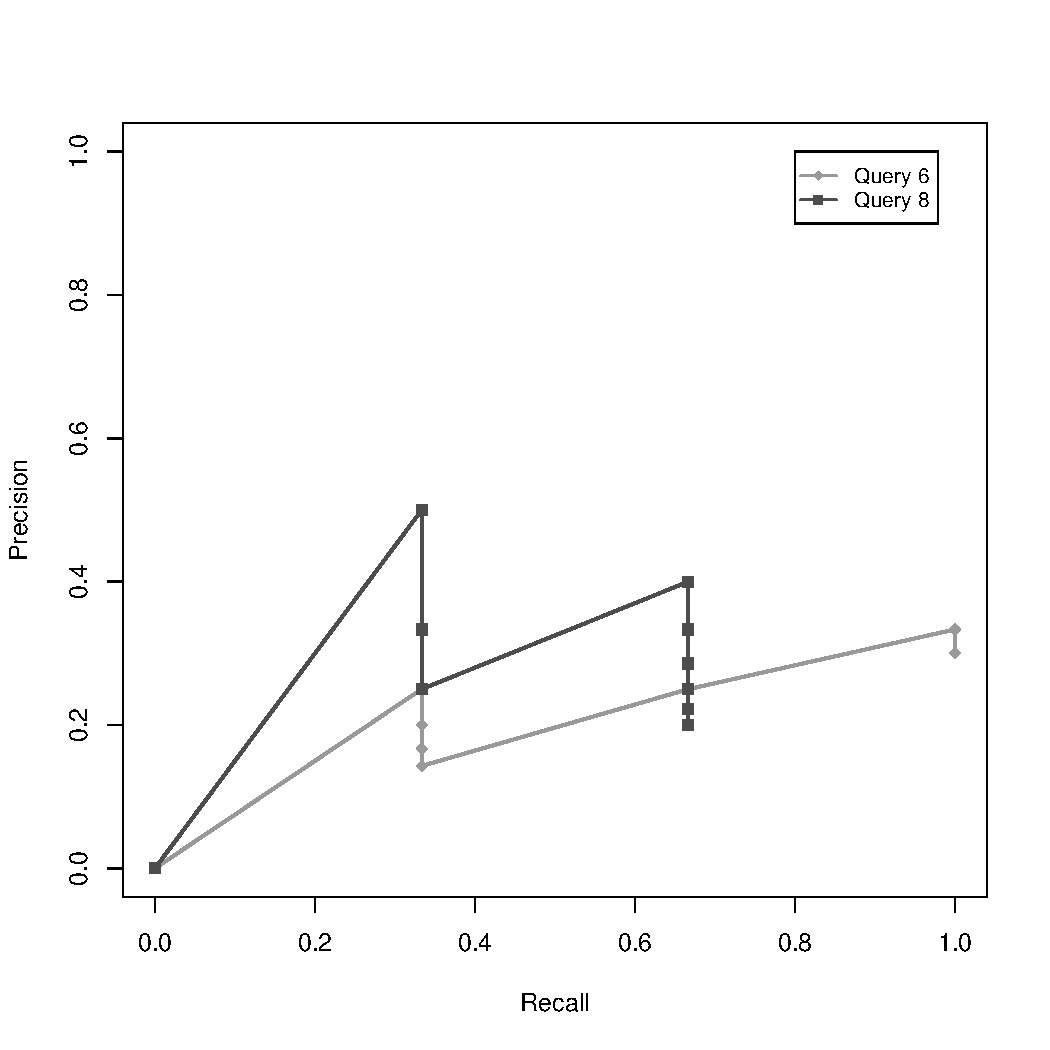
\includegraphics[scale=.6]{code/getrel/urpg68.pdf}
\caption{Uninterpolated Recall-Precision Graph for CACM Queries 6 and 8.}
\end{figure}


\subsubsection{Interpolated Precision}
The graph for the interpolated precision at standard recall values is shown in Figure \ref{fig:iprgraph68} and the table of the values for each query, including the averages, is shown in Table \ref{tab:ipr68}.

\begin{figure}[H]
\centering
\label{fig:iprgraph68}
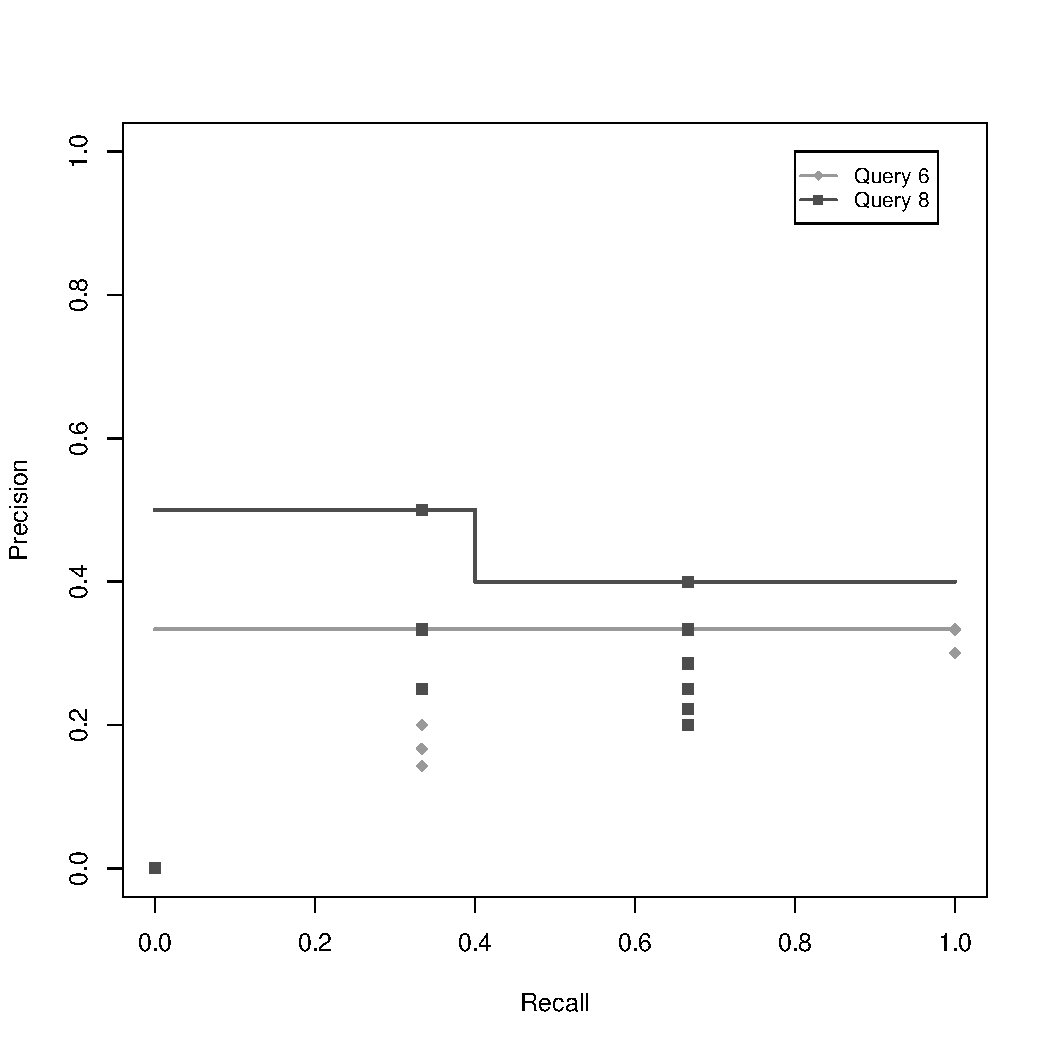
\includegraphics[scale=.6]{code/getrel/ipr68.pdf}
\caption{Graph of interpolated precision at standard recall values for queries 6 and 8.}
\end{figure}

\begin{table}[H]
\centering
\begin{tabular}{ l l l l l l l l l l l l }
Recall & 0.0 & 0.1 & 0.2 & 0.3 & 0.4 & 0.5 & 0.6 & 0.7 & 0.8 & 0.9 & 1.0 \\
\cline{2-12}
Query 6 & 0.333 & 0.333 & 0.333 & 0.333 & 0.333 & 0.333 & 0.333 & 0.333 & 0.333 & 0.333 & 0.333 \\
\cline{2-12}
Query 8 & 0.5 & 0.5 & 0.5 & 0.5 & 0.4 & 0.4 & 0.4 & 0.4 & 0.4 & 0.4 & 0.4 \\
\cline{2-12}
Average & 0.417 & 0.417 & 0.417 & 0.417 & 0.367 & 0.367 & 0.367 & 0.367 & 0.367 & 0.367 & 0.367 \\
\cline{2-12}
\end{tabular}
\caption{Interpolated precision at standard recall values.}
\label{tab:ipr68}
\end{table}

\subsubsection{Average Interpolated Precision}
The graph of the average interpolated precision at standard recall values for queries 6 and 8 can be found in Figure \ref{fig:aiprgraph68}.

\begin{figure}[H]
\centering
\label{fig:aiprgraph68}
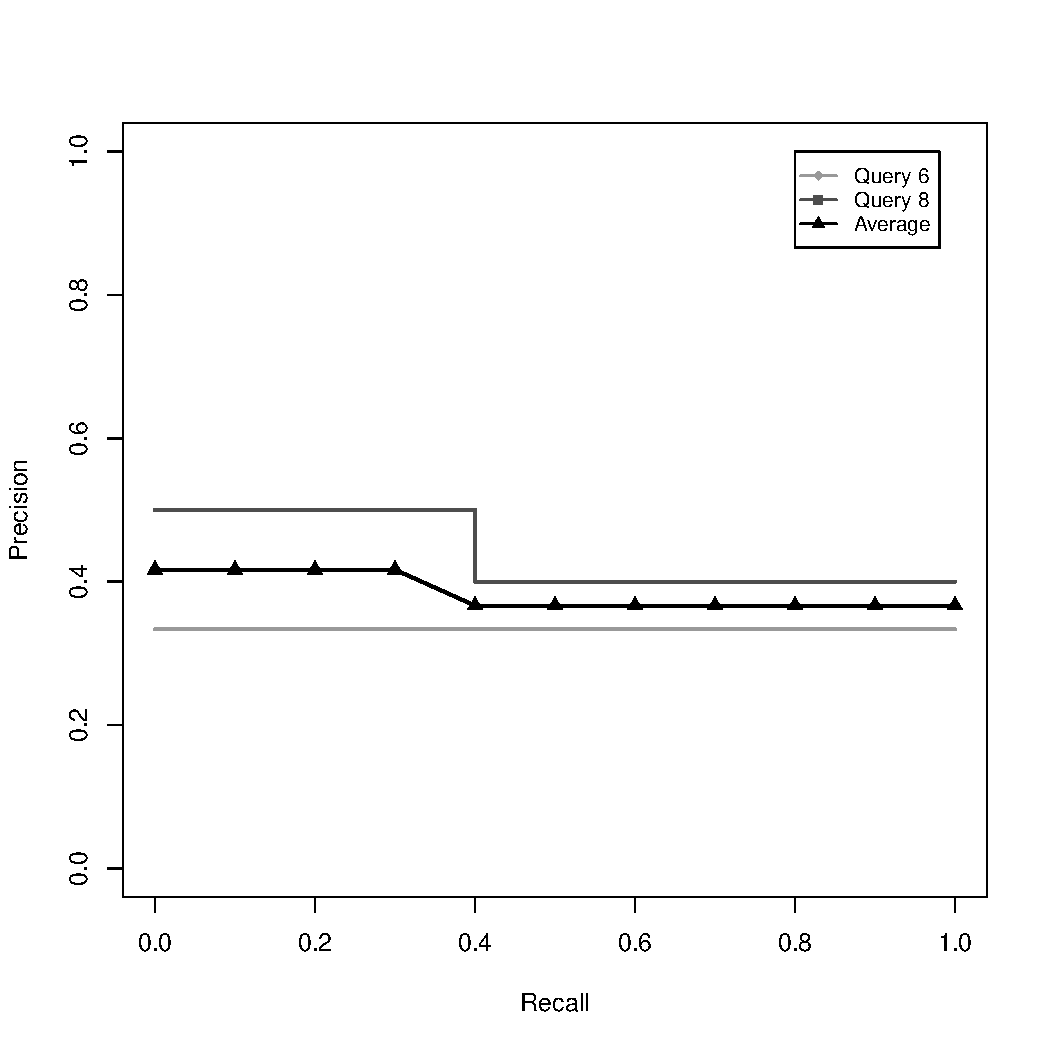
\includegraphics[scale=.6]{code/getrel/aipr68.pdf}
\caption{Average interpolated recall-precision graph for CACM Queries 6 and 8.}
\end{figure}





\section{Appendix} \label{appdx}

\subsection{Code listings}

\lstinputlisting[language=Python, caption={stem.py}, label=listing:stem]{code/stem.py}


\lstinputlisting[language=Python, caption={data.py}, label=listing:data]{code/data.py}

\clearpage

\lstinputlisting[language=Python, caption={cluster.py}, label=listing:cluster]{code/cluster.py}

\lstinputlisting[language=Python, caption={mln1.py}, label=listing:mln1]{code/mln1.py}
\clearpage

\lstinputlisting[language=Python, caption={spelling.py}, label=listing:spelling]{code/spelling.py}
\clearpage

\lstinputlisting[language=Python, caption={calc.py}, label=listing:calc]{code/calc.py}
\clearpage





\bibliography{report}
\bibliographystyle{unsrt}

\end{document}
